% Template for PLoS
% Version 1.0 January 2009
%
% To compile to pdf, run:
% latex plos.template
% bibtex plos.template
% latex plos.template
% latex plos.template
% dvipdf plos.template

\documentclass[10pt]{article}

% amsmath package, useful for mathematical formulas
\usepackage{amsmath}
% amssymb package, useful for mathematical symbols
\usepackage{amssymb}

% graphicx package, useful for including eps and pdf graphics
% include graphics with the command \includegraphics
\usepackage{graphicx}
\usepackage[utf8]{inputenc}
\usepackage[T1]{fontenc}
\usepackage[icelandic,english]{babel}
\usepackage{float}

% cite package, to clean up citations in the main text. Do not remove.
\usepackage{cite}

\usepackage{color} 

% Use doublespacing - comment out for single spacing
%\usepackage{setspace} 
%\doublespacing


% Text layout
\topmargin 0.0cm
\oddsidemargin 0.5cm
\evensidemargin 0.5cm
\textwidth 16cm 
\textheight 21cm

% Bold the 'Figure #' in the caption and separate it with a period
% Captions will be left justified
\usepackage[labelfont=bf,labelsep=period,justification=raggedright]{caption}

% Use the PLoS provided bibtex style
\bibliographystyle{plos2009}

% Remove brackets from numbering in List of References
\makeatletter
\renewcommand{\@biblabel}[1]{\quad#1.}
\makeatother


% Leave date blank
\date{}

\pagestyle{myheadings}
%% ** EDIT HERE **


%% ** EDIT HERE **
%% PLEASE INCLUDE ALL MACROS BELOW

%% END MACROS SECTION

\begin{document}

% Title must be 150 characters or less
\begin{flushleft}
{\Large
\textbf{Measles in small populations : predictability in highly stochastic systems}
}
% Insert Author names, affiliations and corresponding author email.
\\
Q. Caudron$^{1,\ast}$, 
A. S. Mahmud$^{2}$, 
C. J. E. Metcalf$^{1}$,
M. Gottfre{\dh}sson$^3$,
B. T. Grenfell$^{1}$
\\
\bf{1} Department of Ecology and Evolutionary Biology, Princeton University, Princeton, NJ, 08544, USA
\\
\bf{2} Office of Population Research, Woodrow Wilson School of Public and International Affairs, Princeton University, Princeton, NJ, 08544, USA
\\
\bf{3} Landsp\'{i}tali, Hringbraut 101, Reykjav\'{i}k, Iceland
\\
$\ast$ E-mail: qcaudron@princeton.edu
\end{flushleft}













% Please keep the abstract between 250 and 300 words
\section*{Abstract}

A standard assumption in the modelling of epidemic dynamics is that of a certain level of homogeneity. The well-known and oft-used SIR model, arguably the most important compartmental model in theoretical epidemiology, assumes that the disease being modelled is strongly immunising, directly transmitted, and has a well-defined period of infection, in addition to these homogeneity assumptions. Childhood infections, such as measles, are prime examples of diseases that fit the SIR-like mechanism, and these infections have been well studied for many systems. Populations are typically assumed to be large and well-mixed, and the data assumed to contain a high signal-to-noise ratio. Differential equations can then be used to model the disease's dynamics, generally with positive results, both in terms of explaining the underlying mechanisms for infection, and for the prediction of future time series data on disease incidence. Here, we consider a setting where populations are small and heterogeneous, and where the dynamics of infection are driven by extinction-recolonisation events. Using a TSIR model, we fit prevaccination measles incidence and demographic data in Bornholm, the Faroe Islands, and four districts of Iceland, between 1901 and 1965. The datasets for each of these countries suffers from different levels of data heterogeneity and sparsity. We explore the potential for prediction of this model~: given historical incidence data and up-to-date demographic information, and knowing that a new epidemic has just begun, can we predict how large it will be~? We show that, despite a lack of significant seasonality in the incidence of measles cases, and potentially severe heterogeneity at the population level, we are able to estimate the size of upcoming epidemics, conditioned on the first time step, to within reasonable confidence. \textcolor{red}{Predictions are best in localities with low}















\section*{Introduction}

Measles is a highly contagious and strongly immunising infection of the respiratory system \cite{Anderson1991}. Due to its extreme transmissibility, its epidemiology is conditional on the birth of susceptible individuals. As such, the temporal dynamics of measles are typically strongly oscillatory, driven seasonally by the increased contact rate amongst young children during school periods \cite{London1973, Fine1982, Schenzle1984}, assuming the population is large enough to sustain the disease. The critical community size, defined as the size of a population required to sustain the disease at an endemic level, is estimated to be between 250,000 and 500,000 \cite{Bartlett1957, Black1966, Keeling1997}. In large populations, measles has been extensively studied, typically demonstrating biennial dynamics in developed countries prior to the introduction of vaccines \cite{Bolker1995, Grenfell1997}. These modelling efforts are typically based on a class of continuous-time systems of differential equations, such as the SIR and SEIR compartmental models. Mechanistically, these models fit well with infectious such as measles, which have a well-defined infectious period, are directly transmitted, and yield lifelong immunity to those who recover from the infection \cite{Anderson1991}. SIR-like models also assume, however, that the dynamics of the incidence of the disease are fairly smooth, and assume a certain level of homogeneous mixing between individuals in the population. In many large-populations studies, such as in \cite{Bjornstad2002}, these assumptions hold reasonably well~: the populations are large and spatially compact enough to guarantee sufficient mixing within the population and to ensure that the disease remains endemic. 

In small populations, however, the dynamics of measles cases are vastly different. Susceptible individuals accumulate when measles is absent; then, driven by stochastic recolonisation, an epidemic may sweep through a large fraction of the susceptible population very quickly, only to go extinct abruptly as susceptibles become depleted. This results in very sharp, spiky epidemics, whose timing may be impossible to predict, described as Type III by Bartlett \cite{Bartlett1957}. As such, methods typically used in the analysis of time-series or in dynamical systems theory are not adapted to the study of temporal changes of measles incidence in these small populations. Nonetheless, scaling analysis of the sizes and durations of measles epidemics in small populations has revealed that some level of predictability can be found within the statistics of epidemic size and duration distributions, despite the small number of epidemics observed over a given period of time \cite{Rhodes1996a, Rhodes1996b}.

A discrete-time adaptation of SIR-like models was developed by Finkenst\"{a}dt and Grenfell \cite{Finkenstadt2000}. The TSIR model is a simple and computationally inexpensive system of difference equations which can be parameterised against observed incidence time-series, and is able to estimate a non-analytical time-varying contact rate. It has been successfully used in the analysis of seasonal variation of measles in several systems with large populations \cite{Bjornstad2002, Grenfell2002, Glass2003, Metcalf2010}. \textcolor{red}{Is this true ? Any other citations recommended here to show that the TSIR can reproduce dynamics that are difficult to model in continuous-time ?} However, little has been done on applying the TSIR model to small populations, despite being theoretically able to tackle fast dynamics such as large epidemics in subendemic populations. \textcolor{red}{Any suggested improvement to this sentence ? Also, has anything been published on small populations and TSIR ?}

In this paper, we address the question of predictability of measles epidemics in small populations. First, we present data on the demographics and disease incidence in prevaccination-era Bornholm, the Faroe Islands, and four districts in Iceland. Then, we summarise the TSIR model and fit the parameters of the model to the data. After generating predictions for the evolution of each epidemic, we compare the mean predictions with the original time-series, and the predicted size of each observed epidemic.














\section*{Methods}

\subsubsection*{Data}

Measles incidence data were obtained for Iceland, the Faroe Islands, and Bornholm (CONFIRM?), from 1900 to 1965, from \cite{Cliff1981}. For Iceland, this dataset collects monthly figures for measles cases reported in 47 medical districts, originally sourced from \textit{Heilbrig\dh{}issk\'{y}rslur} (Public Health in Iceland). Major revisions to the boundaries of medical districts took place twice during the study period : in 1907 and 1932. For the Faroe Islands and Bornholm, the data were originally published WHERE?. 

Medical Report for the Kingdom of Denmark,
1927-1968, National Health Service of Denmark, Copenhagen

Demographic data for Iceland were obtained from two sources. Annual data on population and number of live births for the entire country were taken from \cite{Cliff1983B}. Decadal population data from 1901 to 1965, for 262 municipalities, were obtained from online publication in \cite{StatsIceland}. Municipality boundaries changed from three to five times during the study period. In addition, many municipalities had missing data. Medical districts and municipalities were matched based on names, and confirmed using latitude and longitudes. Using this procedure, we were able to confidently match four medical districts with municipalities. Several matched districts were discarded either due to missing population data, or lack of confidence in the matching of the geographical boundaries. It is also worth noting that matched medical district -- municipality pairs may not encompass the exact same area, but one may be a (potentially partial) subset of the other. With the data available, we were able to match four district -- municipality pairs~: Akureyri, Reykjav\'{i}k, Hafnarfj\"{o}r\dh{}ur, and Vestmannaeyjar.

Data on the demographics of the Faroe Islands were taken from the Statistical Yearbooks of Denmark published by \cite{StatsDenmark}, and from Statistics Faroe Islands \cite{StatsFaroe}. Annual data on population and births from 1901-1965 were obtained in aggregated form for all of the islands in the Faroe archipelago. 

Demographic data for Bornholm was collected from several publications from \cite{StatsDenmark}. Annual population data for Bornholm were obtained from \cite{StatsDenmark}, which contains detailed statistical information collected by Statistics Denmark. Pre-1930 annual birth data were obtained from the \textit{\AE{}gteskaber, F\o{}dte og D\o{}de} (Marriages, Births and Death) publications of Statistics Denmark. Post-1930 annual birth data were obtained from \textit{Befolkningsudvikling og sundhedsforhold 1901-60} (Population, Development and Health 1901 - 1960), also from Danmarks Statistik.

All locations experienced a slight decline in birth rates just prior to 1940, followed by a sharp increase in births after 1940. In Bornholm, births declined steadily from around 1945 onwards. In Iceland and the Faroe Islands, aggregate births increased steadily from 1940s onwards, with a slight decline in Iceland around 1960.

Figure \ref{figIncidence} shows the reported incidence for Bornholm, the Faroe Islands, and four districts of Iceland.










\subsubsection*{The TSIR model}

For systems with small, heterogeneous populations, epidemic dynamics are driven by stochasticity in the timing of disease recolonisations and in population mixing. As such, dynamical models such as the well established SIR model are unable to adequately represent the underlying biological processes which dictate the evolution of disease incidence over time. The time-series SIR model \cite{Finkenstadt2000} is a discrete-time, stochastic model of disease progression written in terms of a set of difference equations. Assuming that the infection is fully immunising and that the infectious period is well-defined, then the evolution of the number of infected cases, $I$, can be written,
\begin{equation}
\mathbb{E}\left[I_{t+1}\right] = r_t \, S_t \, I_t^\alpha,
\label{TSIR_I}
\end{equation}
where $S_t$ is the number of susceptible individuals at time $t$, seasonal contact rates are represented by the periodic parameter $r_t = r_{t+P}$ for $P$ time steps per year, $0 < \alpha < 1$ is an inhomogeneity parameter, and where $\mathbb{E}\left[\,\cdot\,\right]$ denotes the expectation operator. The time step is set as the generation time of the infection. Then, the number of susceptible individuals is defined by,
\begin{equation}
S_{t+1} = S_t + B_{t-d} - I_t + u_t, \quad \mathbb{E}\left[u_t\right] = 0.
\label{TSIR_S}
\end{equation}
Here, $u_t$ is  zero-mean additive noise. $B_{t-d}$ is the number of births born $d$ time step prior to $t$, the delay $d$ assumed due to maternal immunity, and set at four months \cite{Anderson1991}.

The observed number of cases, $C_t$, is assumed to be underreported by a reciprocal reporting rate $\rho_t \ge 1$, such that the true number of infected cases at time $t$ is given by $I_t = \rho_t \,C_t$. If the number of susceptible individuals $S_t$ fluctuates around a mean $\bar{S}$ such that $S_t = \bar{S} + Z_t$, then, from equation (\ref{TSIR_S}), the dynamics of the susceptible individuals are given by
\begin{equation}
Z_{t+1} = B_{t-d} + Z_{t} - \rho_t\,C_t + u_t.
\label{iter}
\end{equation}
A major assumption made by the TSIR model is that all individuals will eventually become infected. As such, the incidence of infected cases should track births. Successive iteration of equation (\ref{iter}) yields,
\begin{equation}
Z_{t+1} = \sum_{i=1}^t B_{i-d} - \sum_{i=1}^t \rho_i \, C_i + \sum_{i=1}^t u_i + Z_0.
\label{sums}
\end{equation}
If $\rho_t = \rho$ is a constant, and $u_t$ is small, then equation (\ref{sums}) reflects a linear relationship between the cumulative births and the cumulative incidence. However, as $Z_{t+1}$ depends on $Z_t$, it can be shown that the reporting rate need not be a constant, and that it could be estimated using locally linear regression methods. Then, $Z_t$ can be found as the residuals of this regression. 






\subsubsection*{Fitting}

The time step in the difference equations (\ref{TSIR_I}) and (\ref{TSIR_S}) is fixed at the generation time of the infection. For measles, the period of time from infection to recovery is approximately two weeks \cite{Anderson1991}. Due to the very spiky nature of the reported incidence data (whose derivatives are non-smooth due to low sampling rates), interpolation must be done such that peaks in the data are not missed or reduced. As such, a linear interpolant with an integer multiple of the number of points per year was used. This yielded 24 time points per year, thus maintaining the maximum values of the peaks in the data, and fixing the generation time at just over fifteen days.

Population and live births, assumed to be smooth, were interpolated cubically to 24 time points per year. Despite large intervals between some of the reported demographics data, Finkenst\"{a}dt and Grenfell \cite{Finkenstadt2000} report that the regression for reconstructing susceptibles is robust to pronounced changes in birth rates.

The reporting rate $\rho_t$ was estimated using Gaussian process regression, given the births and reported cases. Unlike splines or locally-weighted regression methods, Gaussian process regressions do not optimise smoothness of the fitted values, but instead yield the best unbiased estimates, assuming the error in the underlying process is normally distributed. Once found, $\rho_t$ is the derivative of the Gaussian process prediction for the cumulative number of births, with respect to the cumulative number of cases, and $Z_t$ are the residuals of the regression.

The mean number of susceptibles $\bar{S}$ was estimated marginally by profiling the likelihood of the logarithmic form of equation (\ref{TSIR_I}) :
\begin{equation}
\ln\big(\mathbb{E}\left[I_{t+1}\right]\big) = \ln(r_t) + \ln\left(\bar{S} + Z_t\right) + \alpha \ln\left(I_t\right),
\end{equation}
after which the seasonal contact rates $r_t$ were estimated conditionally on $\bar{S}$. The inhomogeneity parameter was fixed at $\alpha = 0.97$, as in \cite{Metcalf2010}, implying a small, nonlinear inhomogeneity, yet not significantly impacting transmission dynamics between large and small epidemics. \textcolor{red}{Not sure this is relevant here -- there are no epidemic troughs because we just go to zero. Perhaps best to try inferring this once more, now that sensitivity thresholds are better established.}






\subsubsection*{Predictions}

Using the TSIR model as defined by the system of equations (\ref{TSIR_I}, \ref{TSIR_S}), predictions for epidemic dynamics were made by sampling the incidence $I_{t+1}$ from a binomial distribution :
\begin{equation}
I_{t+1} \sim \mathrm{Bin}\left(S_t, \, 1-\mathrm{e}^{-\lambda}\right),
\end{equation}
where the number of Bernoulli trials is given by the number of susceptible individuals, $S_t$. The probability of a successful infection is defined by the force of infection, $\lambda = r_t\,I_t^\alpha$, cumulated over one biweek period. This assumes that each individual spends an exponentially-distributed period of time in the infected class.

Due to the abundance of zeros in the incidence time-series, initial conditions cannot simply be taken as the point $\left(I_0, S_0\right)$. Instead, each epidemic must be simulated independently, with initial conditions given by the data at the time that the epidemic begins. For each epidemic, we fix the number of infected cases and of susceptible individuals as per the data, and allow the simulation to continue until the next epidemic begins. Thus, we always simulate the same number of epidemics as given by the incidence data, where each epidemic is simulated conditioned on the data available at the beginning of that epidemic. \textcolor{red}{Is this clear, or does it need rewording ?}

In order to clearly establish when this time is, a sensitivity threshold must be set. Let $\tau \in \mathbb{Z}^+$ define the number of reported infected cases necessary for any particular biweek period to be considered part of an epidemic. A choice of $\tau = 1$ ensures that all available non-zero data is used. However, many potential epidemics go extinct before propagating through the population, especially in highly heterogeneous populations. As such, using $\tau=1$ would cause a large number of strongly overestimated epidemics, which in turn would deplete the susceptible pool, and underestimate future epidemics. As such, we treat $\tau$ as a sensitivity parameter, and fit it by selecting the sensitivity threshold which yields the highest correlation between the mean predicted epidemic traces and the incidence data, as defined by Pearson's $R^2$. Then, the first point in a sequence of time steps whose incidence is greater than or equal to the threshold is considered the beginning of that epidemic.




















% Results and Discussion can be combined.
\section*{Results}

\subsubsection*{Dynamics}

After fitting parameters as described above, predicted epidemic time-series were generated for each of the six localities, using the sensitivity thresholds reported in Table \ref{tableTau}. The mean of fifty thousand simulations, and the inferred seasonalities, are shown in Figure~\ref{figSims}, with their respective 95\% confidence intervals. The reported zero-corrected correlation coefficient is simply Pearson's $R^2$ computed between the mean prediction and the observed incidences, with points where both time-series are zero left out, to reduce inflation of the correlation due to the large number of zeroes in the time-series. 





A significant number of predicted epidemics have a right shoulder, where the model predicts that epidemics take longer to go extinct than those observed. Depending on locality, many of these shoulders are small (Akureyri, Hafnarfj\"{o}r\dh{}ur, and Vestmannaeyjar), whilst for other localities, predicted epidemics may fail to go extinct entirely, demonstrating cyclical behaviour until the beginning of the next epidemic (Bornholm, the Faroe Islands, and Reykjav\'{i}k). This may indicate that the inhomogeneity parameter, fixed at $\alpha=0.97$ for these simulations, is an overestimate. \textcolor{red}{Thoughts on this ? Inferred values are between 0.8 and 0.92, but resulting predictions are fairly poor.}


The inferred seasonalities have wide distributions, demonstrated by their large confidence intervals. This is potentially due to the highly stochastic nature of measles recolonisations into their respective localities, which is the primary driver for when epidemics occur. \textcolor{red}{Need to expand, or is it clear that this wouldn't be the case in large populations, where measles can be sustained ?}

\textcolor{red}{What else should be said here about Figure~\ref{figSims} ?}





\subsubsection*{Predictability in Epidemic Sizes}

Rather than considering a point-wise comparison between the predicted and observed epidemic time-series, a potentially more robust measure of predictability is the total number of infected cases that a particular epidemic will generate. We define the size of an epidemic as the sum of reported cases $C_t$ for observed data, or $I_t / \rho_t$ for predicted data, from the first time point in an epidemic to the time point before the next epidemic begins. Figure~\ref{fig_sizes} shows the mean predicted epidemic size for each observed epidemic for the six localities. Several of these localities show a strong linear relationship, with near-zero intercepts and gradients around one. \textcolor{blue}{Fill in numbers after simulations.}

\textcolor{red}{Any more to be said in this section ?}




































\section*{Discussion}

Predictions on epidemic sizes can be made with a significant level of certainty, despite sparse demographic data for all localities, mismatching incidence and demography information in Iceland, and strong spatial barriers to population mixing in the Faroe Islands. 


TAU



Interpolated our monthly data for 24 periods - discuss effects of this. Trajectory matching vs simple interpolation.

Reconstructed susceptibles in six small populations ( discuss Sbar / N ).

Inferred reporting rate - may be indicator of bad dataset if above one ?

Low to no seasonal effects found - do we want a histogram of epidemic periods throughout the year ? No relatable seasonal effects within Iceland. Do we prefer 12-period of 24-period seasonality ? Could $r$ be representative of some simply random effect that is not really a seasonal factor ? Can we do as well in predicting using flat $r$ ?

SOME predictability found - given the simple model, we do OK at reconstructing epidemics. Reasonable correlation between the epidemic sizes. Duration much less predictable - possible due to how we define an epidemic and cut them off as they run into the next one.

In all cases, our epidemics are longer in time - we don't go extinct as much as we should. Can we suggest an improvement in the model to ameliorate this ?

Intercept on size plot - we should be seeing zero intercept, gradient one. We're seeing greater gradient, so we're overestimating size; positive intercept may indicate improvement needed in the model





Note Bornholm ( single island, clean data effect ) vs Faroe ( many small islands, aggregate incidence data ) vs Icelandic areas ( disconnected demographics vs incidence borders ). In good locations, we can certainly give a good prediction of epi size. Tend to do better for large epidemics. Gradients all ABOUT one, some slightly over ( right shoulder effect ? ). Large variability in error bars - some epidemics are easier to predict than others ( why ? )




ROMAIN :

Why did this method work on other datasets and not this one ? Demography

What other methods could work on this data ?

What can be done to improve the quality of the data ?






% You may title this section "Methods" or "Models". 
% "Models" is not a valid title for PLoS ONE authors. However, PLoS ONE
% authors may use "Analysis" 
\section*{Materials and Methods}











% Do NOT remove this, even if you are not including acknowledgments
\section*{Acknowledgments}









%\section*{References}
% The bibtex filename
\bibliography{qbib}

\section*{Figure Legends}
%\begin{figure}[!ht]
%\begin{center}
%%\includegraphics[width=4in]{figure_name.2.eps}
%\end{center}
%\caption{
%{\bf Bold the first sentence.}  Rest of figure 2  caption.  Caption 
%should be left justified, as specified by the options to the caption 
%package.
%}
%\label{Figure_label}
%\end{figure}


\section*{Tables}
%\begin{table}[!ht]
%\caption{
%\bf{Table title}}
%\begin{tabular}{|c|c|c|}
%table information
%\end{tabular}
%\begin{flushleft}Table caption
%\end{flushleft}
%\label{tab:label}
% \end{table}



\vspace{0.4cm}
\begin{table}[!h]
\centering
\begin{tabular}{ l  c }
\hline \\[-0.9em]
\textbf{Locality} & {$\mathbf{\tau}$} \\[0.1em]
  \hline \\[-0.9em]                   
  Akureyri & 19 \\[0.1em]
  Bornholm & 15 \\[0.1em]
  Faroe Islands & 15 \\[0.1em]
  Hafnarfj\"{o}r\dh{}ur & 8 \\[0.1em]
  Reykjav\'{i}k & 18 \\[0.1em]
  Vestmannaeyjar \hspace{0.2cm} & 7 \\[0.1em]
  \hline  
\end{tabular}
\caption{Sensitivity thresholds $\tau$ for each locality, fit by maximising the correlation between the mean simulated epidemic time-series and the reported incidence data.}
\label{tableTau}
\end{table}





\section*{Figures}

\begin{figure}[!h]
\centering
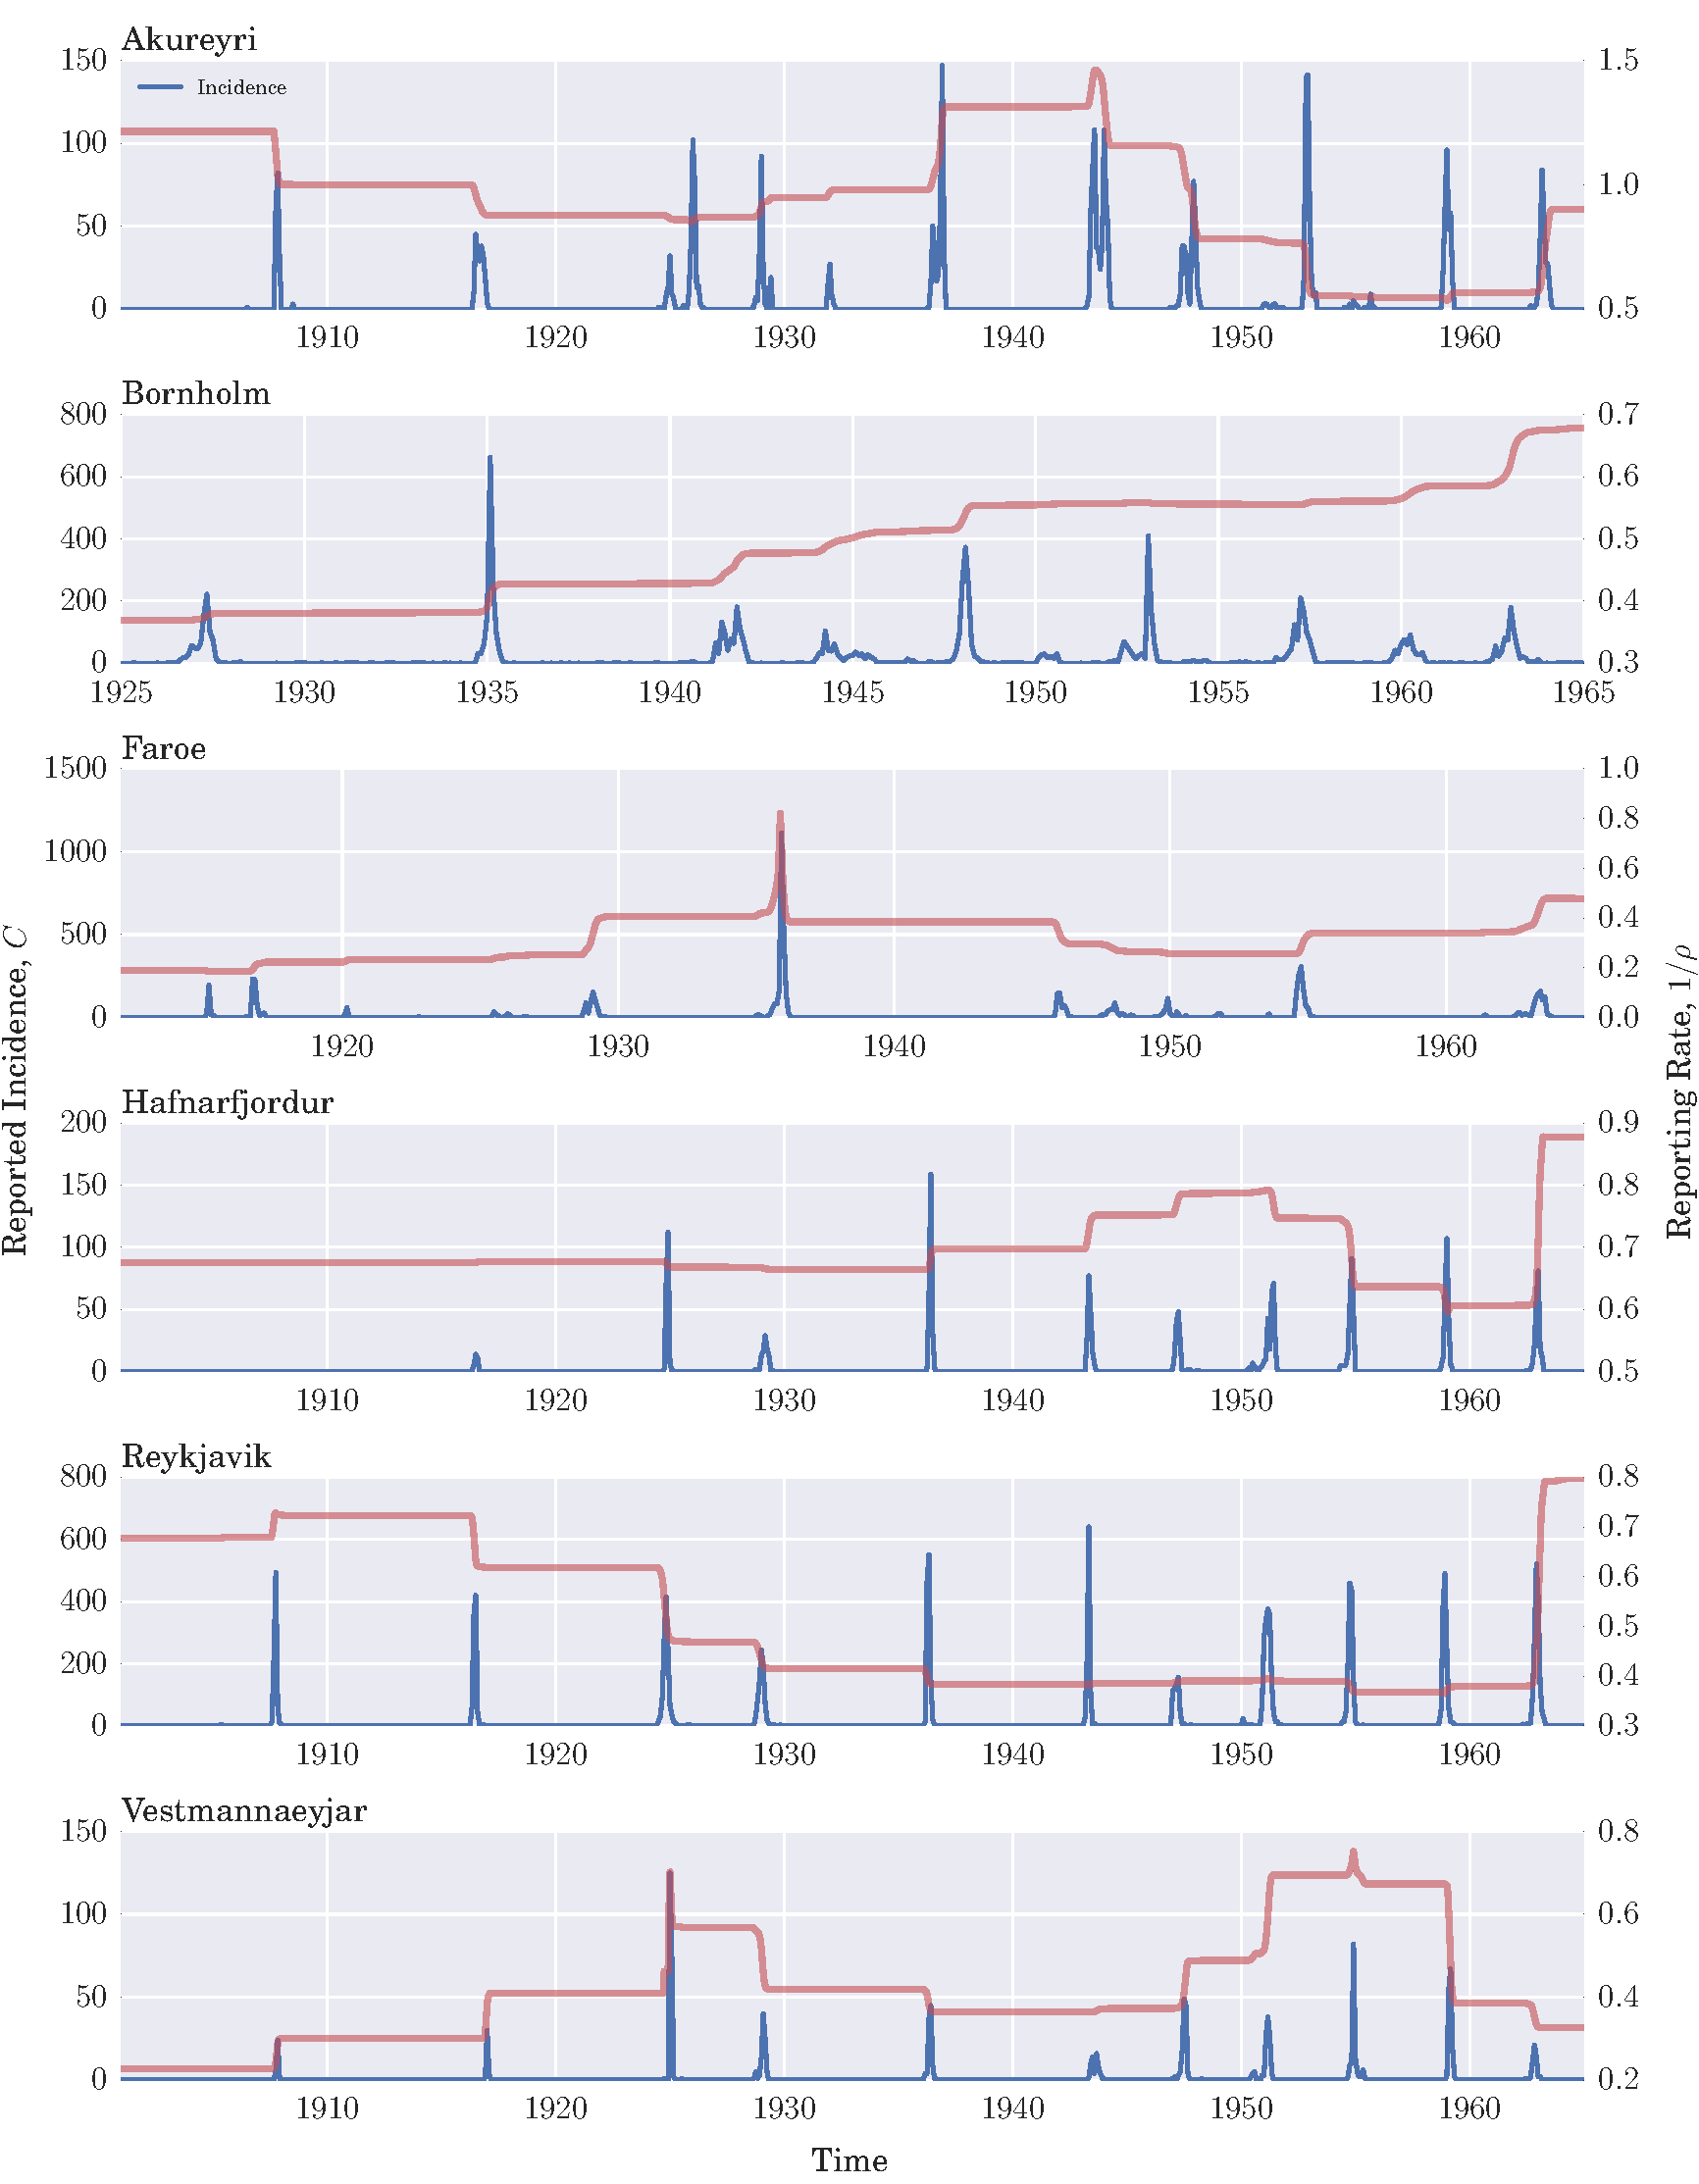
\includegraphics[width=\textwidth]{figures/0_incidence.pdf}
\caption{\textbf{Reported incidence for Bornholm, the Faroe Islands, and four localities in Iceland.} High temporal synchronicity can be seen in the Icelandic localities. }
\label{figIncidence}
\end{figure}



\begin{figure}[!h]
\centering
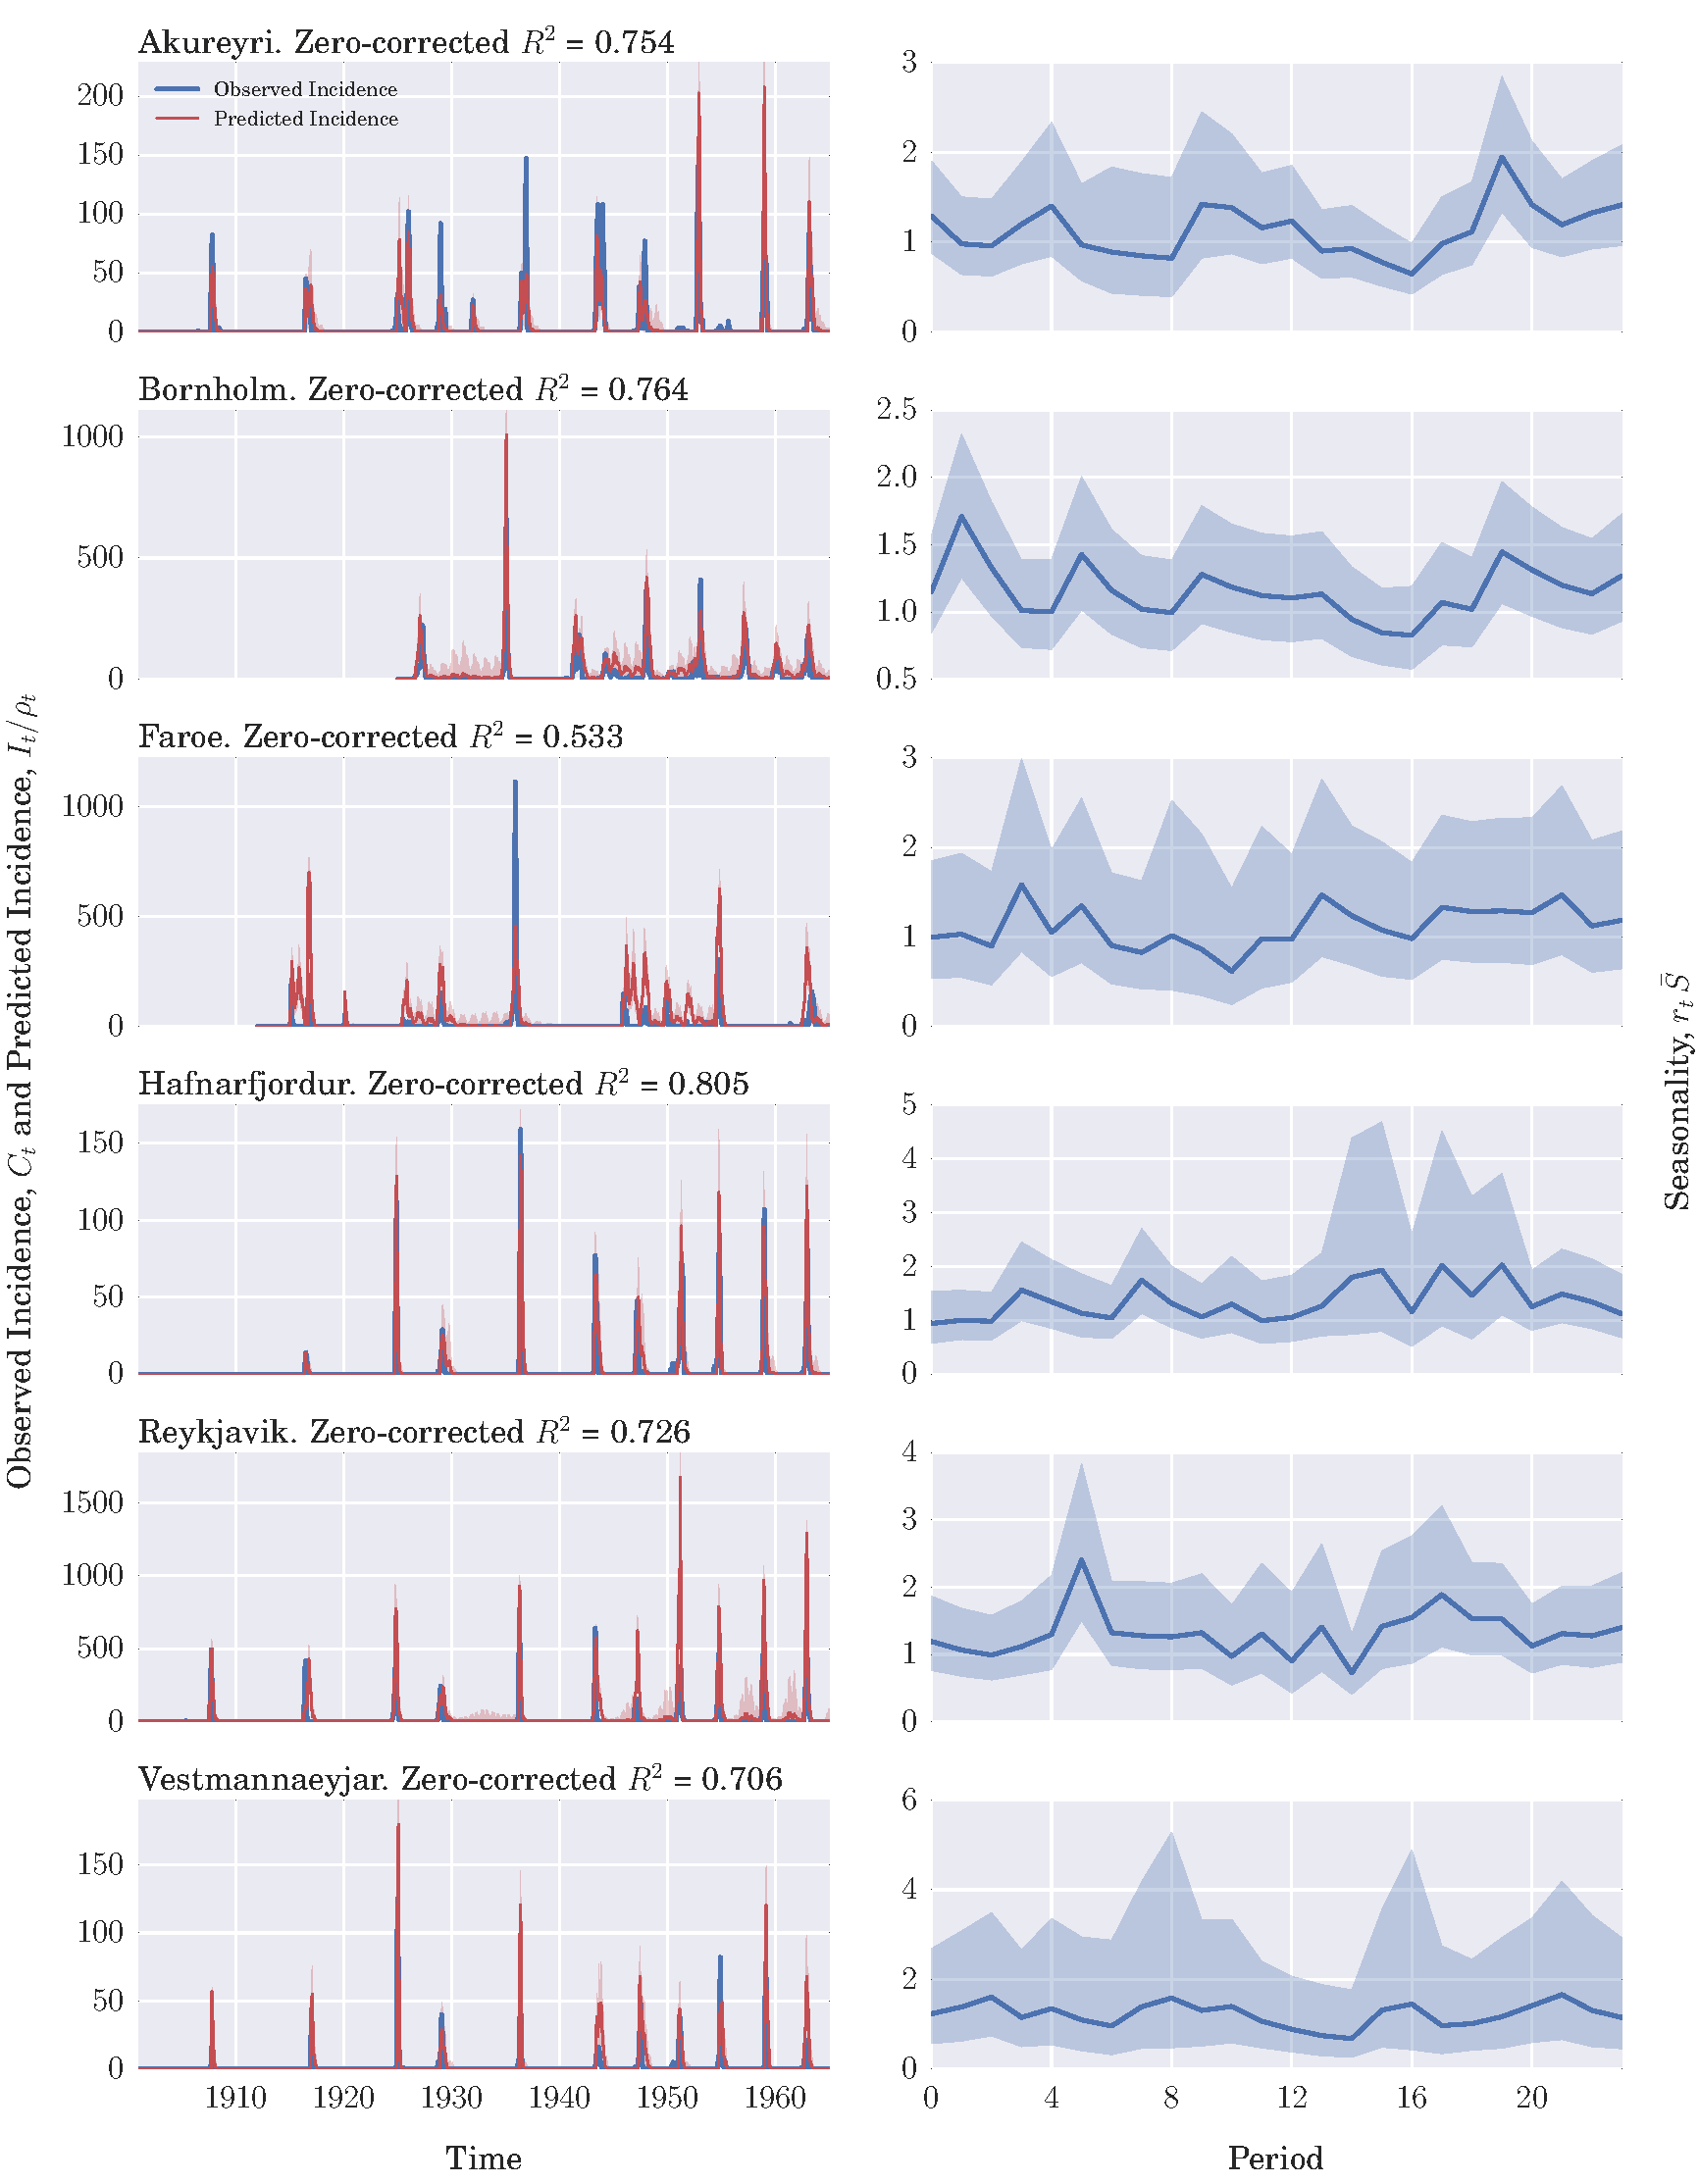
\includegraphics[width=\textwidth]{figures/2_predictions.pdf}
\caption{\textbf{Predicted incidence and inferred seasonal trends.} For the predicted time-series, the mean value of incidence simulations is plotted as a dark red line, with 95\% confidence intervals given in light red. Seasonality is plotted as a function of the biweek, with 95\% confidence intervals in light blue.}
\label{figSims}
\end{figure}


\begin{figure}[!h]
\centering
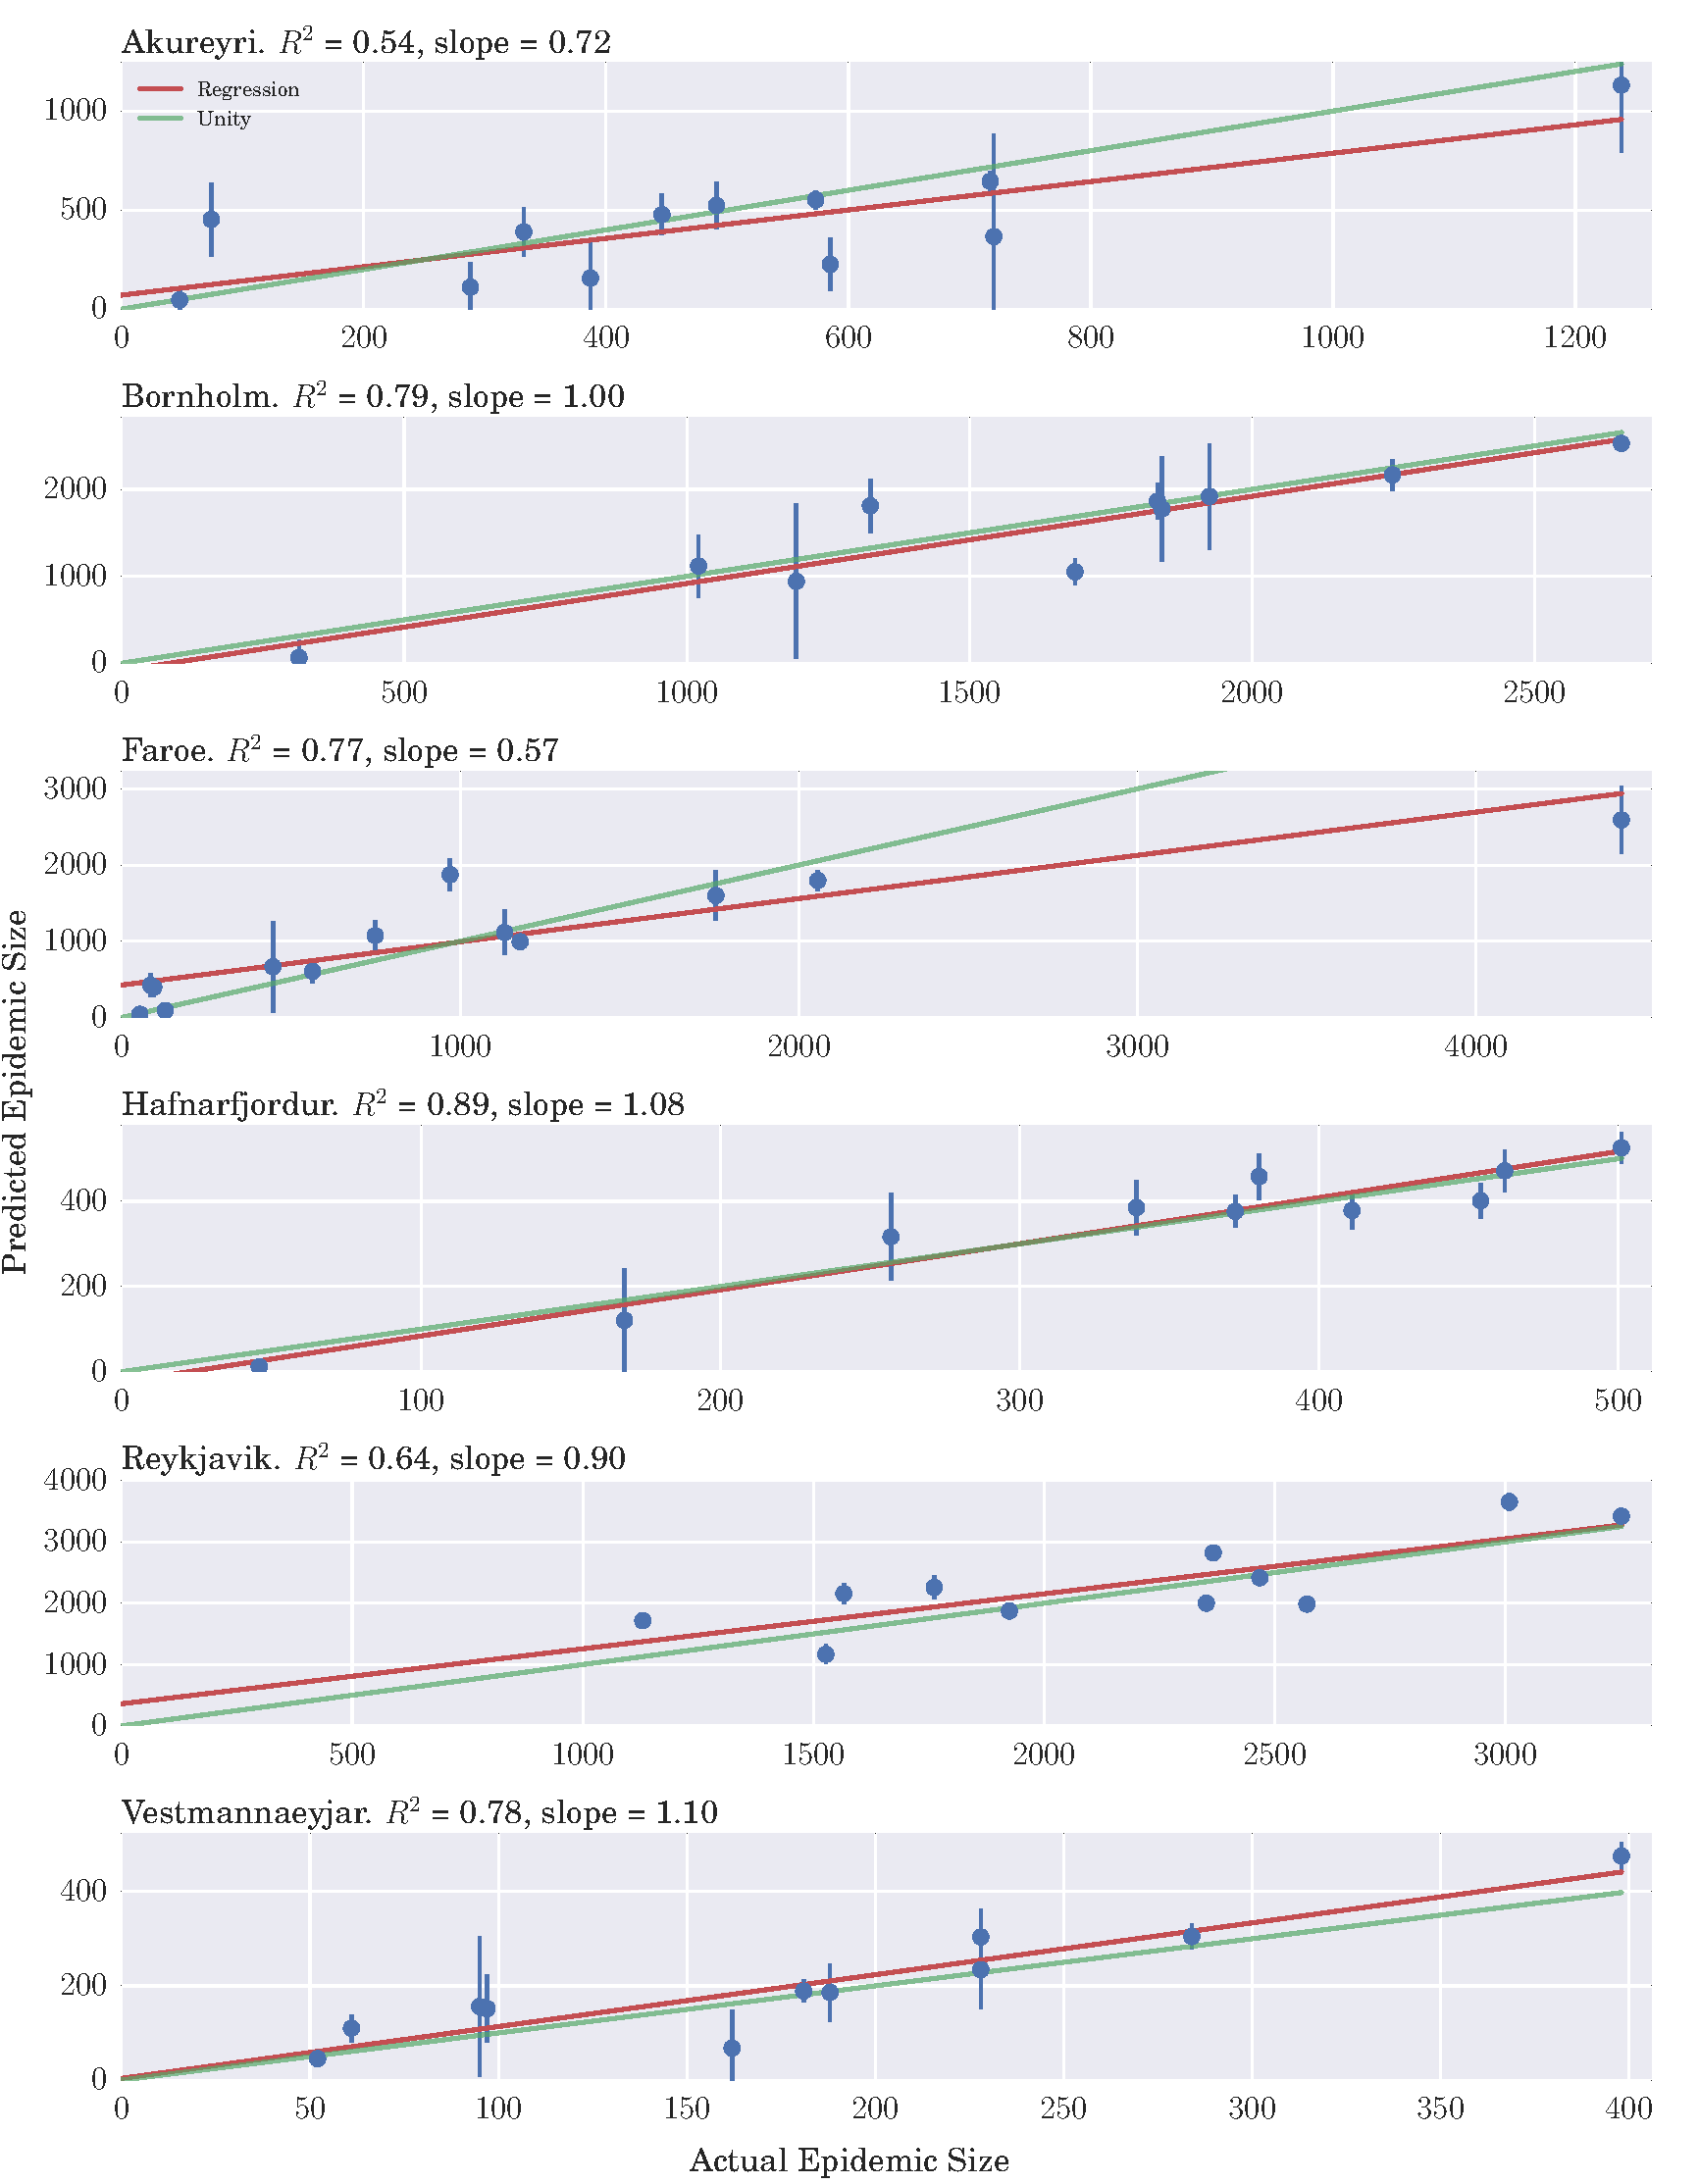
\includegraphics[width=\textwidth]{figures/4_sizes.pdf}
\caption{\textbf{Predictability of epidemic sizes.} The predicted size of each observed epidemic is given as a function of its observed size. \textcolor{red}{Do we want to force the fits through the origin, or report the best regression line with floating intercept as we are now ?}}
\label{fig_sizes}
\end{figure}





\end{document}

